\section{Отношения}

\begin{definition}
\term{Упорядоченным набором}, или же \term{кортежем}, или же \term{отношением}, называется набор объектов, в котором в котором порядок следования элементов имеет значение.
\end{definition}

Для обозначения упорядоченного набора мы будем использовать круглые скобки: $(a, b, \ldots, x)$. Первое отличие упорядоченного набора от множества заключается в упорядоченности элементов, которая отсутствует для множеств. Так в случае множеств $\{a, b\} = \{b, a\}$, но для упорядоченных наборов $(a, b)\not=(b, a)$. Так же в упорядоченных наборах могут встречаться повторения, а в множествах нет. $(a, a)$ является упорядоченным набором, а $\{a, a\}$ множеством не является. Пока отнеситесь к этому просто как к данности, позже будет понятно какой смысл это имеет в приложениях.

Как более-менее практический пример можно рассмотреть базы данных. Чтобы не говорить слишком абстрактно, а рассмотреть более конкретную ситуацию, можно рассмотреть простую записную книжку мобильного телефона, которая тоже по сути является компьютерной базой.

Сама база данных представляет из себя множество записей, каждая из которых состоит из нескольких полей. Пример базы данных представлен в таблице 2.1.

\begin{table}[h]
\centering
\begin{tabular}{lllll}
Фамилия & Имя & Телефон & ДР & Комментарий\\
Авраам & Линкольн & +1(270)... & 12.02.1802 & Президент\\
Бенито & Муссолини & +3(39)... & 29.07.1883 & Фашик\\
Владимир & Ленин & +7(499)... & 22.04.1870 & Свой мужик\\
Григорий & Распутин & +7(3459)... & 21.01.1869 & Есть чему завидовать\\
Джорджина & Байер & +6(64)... & 11.1957 & Транссексуал\\
... & ... & ... & ... & ...
\end{tabular}
\caption{Пример записей в базе данных}
\end{table}

Если предположить, что $F$ — множество фамилий, $N$ — множество имён, $P$ — множество телефонов, $D$ — множество дат календаря и $S$ — множество произвольных текстовых строк, то можно сказать, что данная таблица иллюстрирует множество упорядоченных наборов следующего вида:

$\{(f, n, p, b, c)|f\in F, n \in N, p \in P, b \in D, c \in S\}$

(Строго говоря с точки зрения логики правильнее было бы писать не символ запятой справа в предикате, а символ $\wedge$, но чаще в случаях, подобных нашему, употребляется именно запятая в силу большей наглядности и удобства — означает она при этом логическое И).

Практически вся теория баз данных построена на самом деле на теории множеств в рамках того, что я уже рассказал, и декартова произведения, о котором речь пойдёт ниже. База данных~--- это множество, элементами которого являются упорядоченные наборы. Команды работы с базой данных — это операции, задающие предикаты и операции над множествами. Я не могу позволить себе углубляться сейчас в алгебру реляционных баз данных и синтаксис языка SQL, но вообще рекомендую всем читателям с этими вещами ознакомиться — будет небесполезно, а заодно увидите кучу примеров тому, о чем я сейчас говорю.

Здесь стоит ещё сделать такое наблюдение по терминологии. Чаще всего термин <<кортеж>> применяется именно в теории баз данных, термин <<отношение>> применяется в случае упорядоченных пар, в которых оба элемента принадлежат одному и тому же множеству $\{(x, y)|x\in A, y\in A\}$, а термин <<упорядоченный набор>> используется в остальных случаях. Здесь нет строгого формального разграничения, это просто сложившаяся практика, которая однако может часто нарушаться и в этом нет ничего преступного.

\begin{definition}
\term{Декартовым}, или \term{прямым}, \term{произведением} множеств $A$ и $B$ называется множество $A\times B = \{(a, b)|a\in A, b\in B\}$.
\end{definition}

Говоря человеческим языком, $A\times B$ — это множество всех возможных упорядоченных пар $(a, b)$, таких что $a\in A$ и $b \in B$.

\begin{example}
Пусть $A = \{0, 1\}$, а $B = \{a, b, c\}$. Тогда
$$A\times B = \{(0, a), (0, b), (0, c), (1, a), (1, b), (1, c)\}$$
\end{example}

Кое-какую интуицию относительно декартова произведения вероятно поможет развить иллюстрация в виде таблицы. Столбцы в ней отводятся для элементов одного множества, строки — для другого множества, а на пересечении стоит их декартово произведение. Таблица 2.2 соответствует примеру 2.9.

\begin{table}[h]
\centering
\begin{tabular}{c|ccc}
$\times$ & a&b&c\\
\hline
0 & (0,a) & (0, b) & (0, c) \\
1 & (1, a)& (1, b) &(1, c)
\end{tabular}
\caption{Декартово произведение для примера 2.9}
\end{table}

\begin{example}
Часто с помощью декартова произведения можно описывать какие-то физические понятия. Пусть $A$ — множество мастей (червы, бубны, крести, трефы), а $B$ — множество достоинств (6, 7, 8, ..., король, туз). Тогда $A \times B$ — множество игральных карт в колоде.
\end{example}

\begin{exercise}
Покажите, что в общем случае $A\times B \not = B \times A$. В каких частных случаях все же $A\times B = B \times A$?
\end{exercise}

Легко заметить, что $(A\times B)\times C \not= A\times (B \times C)$, поскольку в случае множества до знака равенства будут получаться пары вида $((a, b), c)$, а для множества справа от знака равенства будут пары $(a, (b, c))$. Однако как и раньше удобно считать, что произведение $A\times B\times C$ без скобок даёт нам упорядоченные тройки $(a, b, c)$ — также без каких-либо специальных группировок. Для удобства часто, впрочем, считают, что и при наличии скобок декартово произведение даёт обычные упорядоченные наборы: 
$$(A\times B)\times C = \{(a, b, c)|a\in A, b\in B, c\in C\}$$

Каждое отношение таким образом является подмножеством декартова произведения $\rho \subset X\times X$ — в этом параграфе нас будут интересовать как раз такие отношения. Часто для удобства применяется следующая запись: если $(x, y) \in \rho$, то пишут $x\rho y$.

\begin{example}
Пусть $S$ — множество высказываний. Тогда любая логическая операция задаёт отношение на этом множестве. В простейшем случае, если рассматривать только одно истинное и ложное высказывание $S = \{0, 1\}$, то $\vee = \{(1, 0), (0, 1), (1, 1)\}$, $\leftrightarrow = \{(0, 0), (1, 1)\}$ и так далее. По аналогии любому предикату на множествах можно сопоставить в соответствие некоторое отношение (возможно, не из двух элементов).
\end{example}

\begin{definition}
Отношение называется \term{рефлексивным}, если для любого $x$ выполняется $x\rho x$.
\end{definition}

\begin{definition}
Отношение называется \term{антирефлексивным}, если для любого $x$ отношение $x\rho x$ не имеет места быть.
\end{definition}

\begin{definition}
Отношение называется \term{транзитивным}, если для любых $x$, $y$ и $z$ из того, что $x\rho y$ и $y \rho z$ следует, что $x\rho z$.
\end{definition}

\begin{definition}
Отношение называется \term{симметричным}, если из того, что $x\rho y$ следует $y\rho x$.
\end{definition}

\begin{definition}
Отношение называется \term{антисимметричным}, если из того, что $x \rho y$ и $y \rho x$ следует, что $x = y$.
\end{definition}

Можно привести и больше возможных общих свойств отношений, но для наших нужд достаточно и того что я уже привёл.

\begin{exercise}
Запишите эти свойства на языке логики.
\end{exercise}

\begin{exercise}
Приведите пример нетранзитивного отношения на множестве $\{0, 1\}$.
\end{exercise}

\begin{definition}
Отношение называется \term{отношением эквивалентности}, если оно рефлексивно, транзитивно и симметрично.
\end{definition}

Отношение эквивалентности часто обозначается символами $=$, $\approx$, $\sim$ и подобными (хотя есть и другие обозначения, которые мы будем по ситуации использовать). Если на множестве задано несколько отношений эквивалентности, то символьное обозначение отношения часто указывается справа внизу от знака эквивалентности: $\approx_R$.

\begin{exercise}
Пусть $S$ — множество учеников средней школы №469. Отношение $x\approx_Y y$ означает, что ученики $x$ и $y$ заканчивают школу в одном году, отношение $x \approx_C y$ означает, что они учатся в одном классе, $x \sim y$ что имеют одинаковую успеваемость. Проверьте, что все заданные отношения — это отношения эквивалентности (для этого необходимо проверить, что они рефлексивны, транзитивны и симметричны).
\end{exercise}

Следующие три упражнения уже посложнее, и их начинающие могут пропустить.

\begin{exercise}
Пусть $S$ — некоторое множество, а $P$ — множество предикатов, определённых на этом множестве. Пусть нам задано такое отношение, что $p \approx q$ тогда и только тогда, когда $p$ и $q$ определяют одинаковые подмножества $S$. Докажите, что это отношение эквивалентности.
\end{exercise}

\begin{exercise}
Пусть нам задано множество логических формул, все с одинаковым числом параметров. Отношение $f=g$ определено для формул, которые на одинаковых значениях параметров принимают одинаковые значения истинности. Докажите, что это отношение эквивалентности.
\end{exercise}

\begin{exercise}
Пусть нам задана некоторая теория. Докажите, что семантическая эквивалентность формул является отношением эквивалентности. (Напомню, что формулы $\phi$ и $\psi$ семантически эквивалентны, если в любой модели теории $\psi\leftrightarrow\phi$).
\end{exercise}

Примеры, приведённые в упражнении, демонстрируют основную идею отношения эквивалентности: это набор пар, которые имеют какие-то общие характеристики, которые и отражают отношение. Причём мыслить об отношении как о парах элементов чаще всего неудобно с интуитивной точки зрения — удобнее мыслить об отношении эквивалентности именно как о наличии какого-то общего свойства.

\begin{definition}
Пусть дано множество $A$ и на нем задано отношение эквивалентности $\sim$. Множество всех элементов $x$, для которых $a\sim x$ называется \term{классом эквивалентности} элемента $a$ и обозначается как $[a]$.
\end{definition}

\begin{thm}
Для любых элементов $a, b \in A$ классы эквивалентности $[a]$ и $[b]$ либо совпадают, либо не пересекаются.
\end{thm}
\begin{proof}
Проведём доказательство от противного и предположим, что теорема неверна. Пусть классы эквивалентности $[a]$ и $[b]$ пересекаются, но не совпадают. Тогда найдётся элемент $x$, принадлежащий сразу обоим классам эквивалентности, и элемент $b' \in [b]$, такой что $b' \not\in [a]$. Для него однако верно, что $b' \sim x$, но поскольку $x \in [a]$ и $x\sim a$, то в силу транзитивности $b' \sim a$ и соответственно $b' \in [a]$. Полученное противоречие говорит, что наше предположение «от противного» было не верно, и значит теорема верна.
\end{proof}

Это доказательство на первый взгляд может показаться странным и непонятным — вспомните тогда свойства импликации и как она связана с выводимостью (см.~\S\S1.5,~1.7):
$$(a\rightarrow b) \leftrightarrow (\neg b \rightarrow \neg a)$$

Смыслом теоремы является тот факт, что каждое множество с заданным на нем отношением эквивалентности можно разбить на непересекающиеся классы эквивалентности.

\begin{example}
Пусть опять $S$ — множество учеников школы №469. Всех учеников можно сгруппировать по классам, по успеваемости или по году окончания школы. Пусть $A$ — множество двоечников, $B$ — троечников, $C$ — хорошистов и $D$ — отличников. Очевидно, что эти множества не пересекаются и $S = A\cup B\cup C\cup D$, причём любые два ученика из одного и того же множества находятся в отношении $\sim$ («имеют одинаковую успеваемость») друг с другом, а ученики из разных множеств в этом отношении не находятся.
\end{example}

\begin{definition}
Процесс разбиения множества на классы эквивалентности называется \term{факторизацией}, а само множество классов эквивалентности называется \term{фактор-множеством}. Если $\rho$ — отношение эквивалентности на $A$, то фактормножество $A$ по $\rho$ обозначается как $A/\rho$.
\end{definition}

\begin{example}
Продолжая пример с успеваемостью, можно записать, что $S/\sim = \{A, B, C, D\}$.
\end{example}

Обратите внимание в какую сторону рисуется черта фактормножества и не путайте её с разностью множеств. $A\setminus B$ — разность, а $A/\rho$ — факторизация.

Интуитивно таким образом можно рассматривать факторизацию как разбиение множества на подмножества в соответствии с некоторым отношением («фактором»). Обратное кстати тоже верно — если множество разбито на непересекающиеся подмножества, то по ним можно задать отношение эквивалентности.

\begin{exercise}
Пусть $A = \{a, b, c, d\}$ разбито на подмножества $\{a, b\}$ и $\{c, d\}$. Запишите по этому разбиению отношение эквивалентности $\rho$ как множество упорядоченных пар (начинается эта запись как $\rho = \{(a, a), (a, b), \ldots\}$).
\end{exercise}

Перейдём теперь ко второму не менее важному типу отношений, которые мы часто будем использовать.

\begin{definition}
	Отношение называется \term{предпорядком}, если оно транзитивно и рефлексивно.
\end{definition}

\begin{definition}
Отношение называется \term{отношением частичного порядка} (или \term{отношением нестрогого частичного порядка}), если оно рефлексивно, транзитивно и антисимметрично.
\end{definition}

\begin{definition}
Отношение называется \term{отношением строгого частичного порядка}, если оно антирефлексивно, транзитивно и антисимметрично.
\end{definition}

Отношение частичного порядка удобно обозначать как $\le$. Отношение строгого частичного порядка — как $<$. Если $a \le b$ и $a \not= b$, то $a<b$. Если $b \le a$, то можно писать $a \ge b$ или $a > b$, если $a\not= b$. Легко видеть, что отношения частичного и строгого частичного порядка — это фактически одного и то же. Различаются они лишь тем, находится ли каждый элемент в отношении с самим собой (то есть можем ли мы записать отношение $x\le x$). В теории в основном используется отношение частичного порядка, в конкретных задачах часто может оказаться удобным и то и другое. Хотя погоды это разграничение не делает: если у нас есть строгий порядок, то его всегда можно сделать нестрогим, дополнив парами $x\le x$, и наоборот нестрогий порядок можно сделать строгим, выкинув такие пары.

\begin{exercise}
Докажите, что если элементами множества являются множества (например, это булеан), то отношение $\subset$ является отношением частичного порядка.
\end{exercise}

\begin{exercise}
Докажите, что отношение «является предком» на множестве людей является строгим частичным порядком.
\end{exercise}

\begin{exercise}
Докажите, что отношение «не ниже чем» на множестве всех людей образует нестрогий частичный порядок, а отношение «выше чем» строгий частичный порядок.
\end{exercise}

\begin{exercise}
Покажите, что отношение «является родителем» не является отношением частичного порядка.
\end{exercise}

\begin{exercise}
Покажите, что на множестве картонных коробок отношение «влезает в» является отношением строгого частичного порядка.
\end{exercise}

\begin{exercise}
Рассмотрим множество всех логических функций с одинаковым числом параметров. Определим на них отношение следующим образом: $f\le g$ тогда и только тогда, когда на одинаковых наборах параметров либо эти функции принимают одинаковое значение, либо $f=0$, а $g=1$. Докажите, что это отношение частичного порядка. Как оно соотносится с порядком на булеане множества?
\end{exercise}

\begin{example}
В микроэкономике рассматриваются отношения предпочтений, задаваемые на множествах альтернатив (читай товаров). Считается, что потребители могут сравнивать альтернативы по степени предпочтительности и данное отношение является как раз отношением частичного порядка. (Психологи однако доказывают, что предпочтения людей не являются рациональными и таким образом не образуют частичный порядок на множестве товаров).
\end{example}

Отношение частичного порядка удобно представлять в виде диаграмм. В качестве примера на рисунке 2.2 представлена диаграмма отношения <<является подмножеством>> для булеана $\{x, y, z\}$. На рисунке стрелка обозначает отношение «является подмножеством». Элементы, располагающиеся выше, оказываются «больше» элементов, располагающихся внизу, если между ними есть путь из стрелок. Если на диаграмме есть стрелка $a\to b$ и стрелка $b\to c$, то по транзитивности должна быть и стрелка $a\to c$, которая не указывается, чтобы не загромождать картинку.

\begin{figure}[h]
\centering
\begin{tikzpicture}
\tikzstyle{set_node}=[ellipse,draw];
\node [set_node] (xyz) at (0,4) {\{x, y, z\}};
\node [set_node] (xy) at (-3,2) {\{x, y\}};
\node [set_node] (xz) at (0,2) {\{x,z\}};
\node [set_node] (yz) at (3,2) {\{y,z\}};
\node [set_node] (vx) at (-3,0) {\{x\}};
\node [set_node] (vy) at (0,0) {\{y\}};
\node [set_node] (vz) at (3,0) {\{z\}};
\node [set_node] (v0) at (0,-2) {$\varnothing$};

\draw[->]  (xy) edge (xyz);
\draw[->]  (xz) edge (xyz);
\draw[->]  (yz) edge (xyz);
\draw[->]  (vx) edge (xy);
\draw[->]  (vy) edge (xy);
\draw[->]  (vz) edge (xz);
\draw[->]  (vx) edge (xz);
\draw[->]  (vy) edge (yz);
\draw[->]  (vz) edge (yz);
\draw[->]  (v0) edge (vx);
\draw[->]  (v0) edge (vy);
\draw[->]  (v0) edge (vz);
\end{tikzpicture}
\caption{Отношение <<подмножество>> на $2^{\{x, y, z\}}$.}
\end{figure}

Отношение частичного порядка таким образом упорядочивает элементы множества. Существенно, однако, что если задан частичный порядок, то совершенно не факт, что удастся сравнить произвольные два объекта. Как видно из диаграммы выше, элементы $\{x, y\}$ и $\{z\}$ несравнимы между собой. Точно так же для любых двух людей не обязательно кто-то один из них должен быть предком другого, и в этом смысле несравнимыми являются брат и сестра.

\begin{definition}
\term{Линейным порядком} называется отношение частичного порядка, относительно которого сравнимы любые два элемента множества.
\end{definition}

\begin{example}
Отношение «не ниже чем» является линейным порядком на множестве людей.
\end{example}

\begin{definition}
\term{Максимальным элементом} называется такой элемент, что не существует элемента, большего него.
\end{definition}

\begin{definition}
\term{Наибольшим элементом} называется такой элемент, что он больше любого другого элемента.
\end{definition}

\begin{example}
На множестве коробок максимальным элементом будет коробка, которая не может влезть ни в какую другую коробку. Наибольшим элементом будет коробка, в которую может поместиться любая другая коробка.
\end{example}

В полной аналогии можно ввести понятия \term{минимального} и \term{наименьшего элемента}, но мы не будем на это отвлекаться, так там вся теория совершенно аналогична.

Очевидно, что если множество обладает наибольшим элементом, то он же будет и единственным максимальным элементом. Однако же максимальных элементов может быть несколько, и наибольшего элемента в этом случае не будет, как в случае диаграммы~2.3, на которой имеется два разных максимальных элемента $e$ и $f$, но нет наибольшего элемента. На диаграмме~2.4 максимальный элемент уже один, он же является наибольшим.

\begin{figure}[h]
\centering
\begin{picture}(120,60)
\put(0,0){a}
\put(40,0){b}
\put(20,50){e}
\put(22,45){\line(-1,-2){18}}
\put(22,45){\line(1,-2){18}}
\put(80,0){c}
\put(120,0){d}
\put(100,50){f}
\put(102,45){\line(-1,-2){18}}
\put(102,45){\line(1,-2){18}}
\end{picture}
\caption{Отношение с несколькими максимумами.}
\end{figure}

\begin{figure}[h]
\centering
\begin{picture}(120,100)
\put(0,0){a}
\put(40,0){b}
\put(20,50){e}
\put(22,45){\line(-1,-2){18}}
\put(22,45){\line(1,-2){18}}
\put(80,0){c}
\put(120,0){d}
\put(100,50){f}
\put(102,45){\line(-1,-2){18}}
\put(102,45){\line(1,-2){18}}
\put(60,90){g}
\put(62,85){\line(-1,-1){40}}
\put(62,85){\line(1,-1){40}}
\end{picture}
\caption{Отношение с наибольшим элементом.}
\end{figure}

В обоих этих примерах порядки не являлись линейными. В случае же линейного порядка, очевидно, что понятия максимального и наибольшего элемента совпадают.

\begin{definition}
\term{Верхней гранью} подмножества $S\subset U$ называется такой элемент $x\in U$, что для любого элемента $s\in S$ выполняется $s \le x$.
\end{definition}

\begin{definition}
\term{Нижней гранью} подмножества $S\subset U$ называется такой элемент $x\in U$, что для любого элемента $s\in S$ выполняется $s \ge x$.
\end{definition}

Если $x$ — верхняя грань подмножества $S$, то любой элемент больший $x$ так же будет являться верхней гранью $S$. Таким образом, верхние грани сами по себе образуют множество (аналогично с нижними) и есть смысл ввести следующие определения:

\begin{definition}
\term{Наименьшей}, или \term{точной}, \term{верхней гранью}, называется наименьшая из верхних граней. Обозначается она как $\sup S$.
\end{definition}

\begin{definition}
\term{Наибольшей}, или \term{точной}, \term{нижней гранью}, называется наибольшая из нижних граней. Обозначается она как $\inf S$.
\end{definition}

(С этого места начинаются абстракции, которые начинающему читателю вероятно и не являются необходимыми — если будет непонятно о чем речь, можно смело пропускать. Если однако разобраться с материалом, то это будет хорошим упражнением для ума.)

Если подмножество $S$ состоит лишь из двух элементов, то операции «точных граней» можно рассматривать как арифметические операции над этими элементами. В этом случае используется запись $\sup\{a, b\} = a\vee b$ и $\inf\{a, b\} = a\wedge b$.

\begin{exercise}
Докажите, что на булеане относительно порядка, образованного включением множеств, $A\wedge B = A\cap B$ и $A\vee B = A \cup B$ и они обладают соответственно всеми свойствами логического И и логического ИЛИ.
\end{exercise}

Сформулированное в упражнении утверждение в общем случае неверно, если рассматривать произвольный частичный порядок. Во-первых, могут не выполняться сами свойства логических операций, а во-вторых самих точных граней может и не быть. Поэтому вводятся следующие определения:

\begin{definition}
\term{Решёткой} называется частично упорядоченное множество, у которого для любого двухэлементного подмножества существуют точные верхние и нижние грани.
\end{definition}

\begin{definition}
\term{Дистрибутивной решёткой} называется решётка, для которой оказываются верны свойства дистрибутивности операций $\wedge$ и $\vee$ (см.~теорему~1.1).
\end{definition}

\begin{exercise}
Докажите, что решётка на диаграмме 2.5 не является дистрибутивной.
\end{exercise}

\begin{figure}[h]
\centering
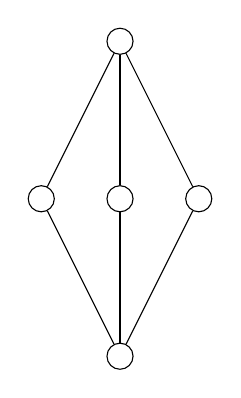
\begin{tikzpicture}
\node[circle,draw] (v5) at (1,0) {};
\node[circle,draw] (v2) at (-1,0) {};
\node[circle,draw] (v1) at (0,2) {};
\node[circle,draw] (v3) at (0,-2) {};
\node[circle,draw] (v4) at (0,0) {};
\draw  (v3) edge (v2);
\draw  (v3) edge (v4);
\draw  (v3) edge (v5);
\draw  (v4) edge (v1);
\draw  (v2) edge (v1);
\draw  (v5) edge (v1);
\end{tikzpicture}
\caption{Недистрибутивная решётка}
\end{figure}

Дистрибутивные решётки уже практически дублируют законы логики, которым была посвящена первая глава. Недостаёт только $1$ и $0$. Следующие определения исправляют ситуацию:

\begin{definition}
Решётка называется \term{ограниченной}, если в ней существуют наибольший и наименьший элементы, обозначаемые соответственно как $0$ и $1$.
\end{definition}

\begin{exercise}
Если решётка имеет минимальный или максимальный элементы, то они будут единственны и будут являться наименьшим и наибольшим элементами. Докажите это.
\end{exercise}

\begin{definition}
\term{Дополнением} элемента $x$ ограниченной решётки называется такой элемент $y$, что $x\wedge y = 0$ и $x \vee y = 1$. Дополнение $x$ обозначается как $\neg x$.
\end{definition}

\begin{definition}
Если в решётке каждый элемент обладает дополнением, то такая решётка называется \term{решёткой с дополнением}.
\end{definition}

\begin{definition}
\term{Булевой алгеброй} называется дистрибутивная решётка, обладающая наименьшим и наибольшим элементами (обозначаемыми соответственно $0$ и $1$).
\end{definition}

\begin{example}
Если рассмотреть двухэлементное множество $\{0, 1\}$ и определить на нем порядок $0 < 1$, то мы получим в точности классическую логику, которую рассматривали в первой главе, которая, как мы теперь знаем, является разновидностью булевой алгебры.
\end{example}

\begin{example}
Булеан любого множества $A$ задаёт булеву алгебру относительно включения множеств, где наибольшим элементом является само множество $A$, а наименьшим пустое множество.
\end{example}

\begin{exercise}
Для булевых алгебр справедливы все законы логики, которые мы приводили в теореме 1.1. Докажите это.
\end{exercise}

Если у нас есть два частично упорядоченных множества $A$ и $B$, то на их декартовом произведении можно задать частичный порядок несколькими способами:

\begin{definition}
\term{Лексикографическим порядком} на $A\times B$ называется порядок, при котором $(a, b) \le (a', b')$ либо когда $a < a'$, либо когда $a=a'$ и $b\le b'$.
\end{definition}

\begin{definition}
\term{Естественным порядком} на $A\times B$ называется порядок, при котором $(a, b) \le (a', b')$ тогда и только тогда, когда одновременно $a \le a'$ и $b \le b'$.
\end{definition}

Оба этих порядка естественно распространяются на декартово произведение любого количества множеств.

\begin{exercise}
 Пусть $B = \{0, 1\}$ и на нем введён порядок $0 < 1$. Будем рассматривать множество $B\times B\times \ldots \times B$ (фактически упорядоченные наборы единиц и нулей) с естественным частичным порядком. Докажите, что такой частичный порядок задаёт булеву алгебру (кстати, как раз ту самую, которая повсеместно используется в программировании и называется там побитовыми логическими операциями).
\end{exercise}

\begin{exercise}
Докажите, что линейно-упорядоченное множество является дистрибутивной решёткой, и соответственно при наличии наименьшего и наибольшего элемента является булевой алгеброй.
\end{exercise}

\begin{exercise}
Является ли булевой алгеброй множество $B\times B \times \ldots \times B$, введённое выше, относительно лексикографического порядка?
\end{exercise}

\begin{exercise}
Пусть теперь $B$ — некоторая произвольная булева алгебра. Является ли булевой алгеброй $B\times \ldots \times B$ относительно лексикографического порядка? А относительно естественного порядка?
\end{exercise}